% OK !
\chapter{Introduction}

\section{Contexte}

Dans le cadre de ma 4\up{ème} année d'études à Polytech Grenoble en informatique, j'ai effectué mon stage de 12 semaines à \textit{Universiti Teknologi PETRONAS (UTP)} à Seri Iskandar, en Malaisie. Ce stage s'est déroulé du \textbf{20 mai 2019} au \textbf{9 août 2013}.

À l'occasion de la mise en place d'un futur partenariat entre \textit{Polytech Grenoble} et \textit{UTP}, différents sujets de stage nous ont été transmis par le bureau des relations internationales de Polytech. Au final, nous sommes partis à quatre : j'ai été accompagné de deux autres étudiants venant de la spécialité INFO (Informatique) et un étudiant d'IESE (Informatique et Électronique des Systèmes Embarqués).


\begin{figure}[h]
  \centering
  \begin{subfigure}{.5\textwidth}
    \centering
    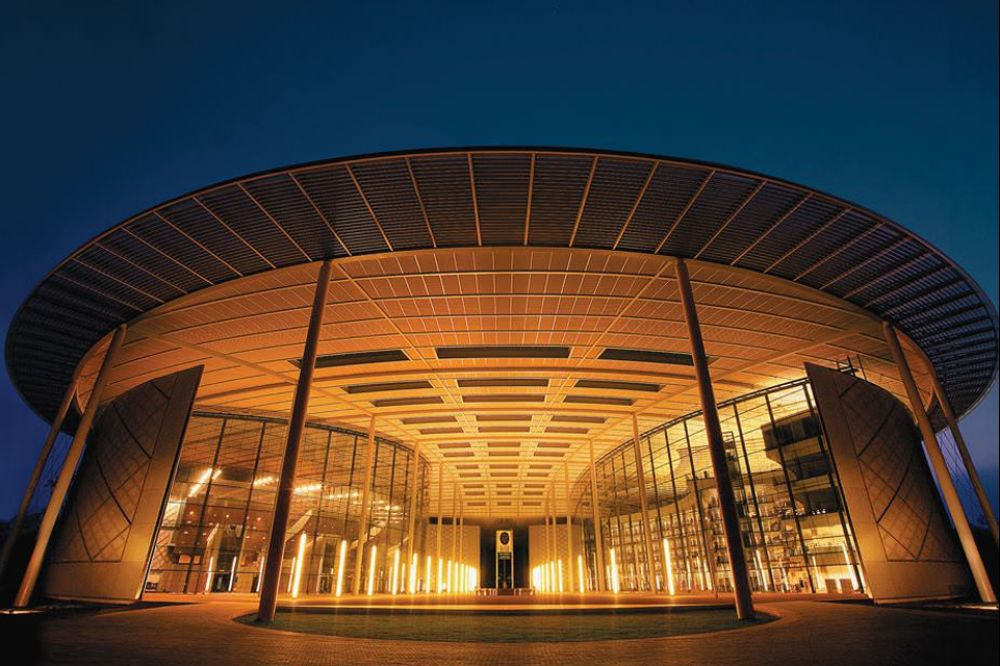
\includegraphics[width=.8\linewidth]{content/imgs/utp.jpg}
    \caption{Bibliothèque de l'université}
  \end{subfigure}%
  \begin{subfigure}{.5\textwidth}
    \centering
    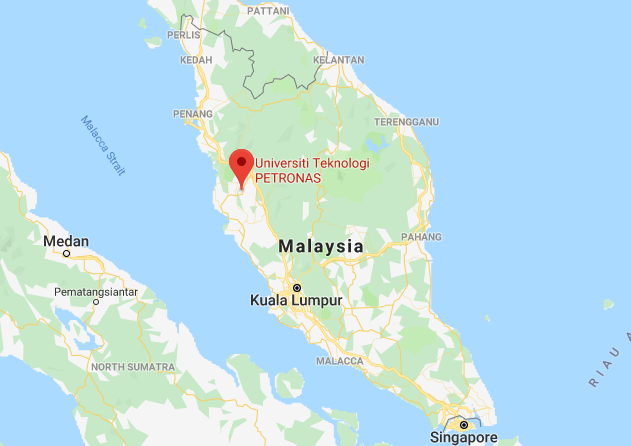
\includegraphics[width=.8\linewidth]{content/imgs/map.png}
    \caption{UTP, Seri Iskandar, Malaisie}
  \end{subfigure}
  \caption{Universiti Teknologi PETRONAS}
\end{figure}




\section{Sujet proposé}

Le sujet qui m'a été proposé a pour objectif de développer une application mobile dont le but est d'aider les personnes atteintes de bégaiement à guérir.

D'après \textit{Wikipédia}\cite{def_wiki}, le bégaiement est un trouble de la parole affectant le débit de la parole caractérisé par des répétitions et prolongations involontaires des sons, syllabes, mots ou phrases, et par des pauses silencieuses involontaires dans lequel le « bègue » (terme désignant un individu souffrant de bégaiement) est incapable de produire un son.

Une application similaire a déjà été développée durant trois années par des étudiants dans le cadre de leurs projets de fin d'études. Tel qu'illustré dans l'annexe \ref{appendix:old_app}, cette application propose les fonctionnalités suivantes :

\begin{itemize}
  \item Des exercices pour apprendre à contrôler son flux de parole ;
  \item La possibilité de visualiser sa progression pour chaque exercice (sous forme de liste, et pour certain exercices sous forme de graphique) ;
  \item Des informations concernant le bégaiement.
\end{itemize}

Cette application était disponible sur les appareils \textit{Android} via le \textit{Play Store}, la plateforme de téléchargement d'applications développée par \textit{Google}. Suite à un trop grand nombre de retours de \textit{bugs} concernant l'application, celle-ci a dû être retirée du \textit{Play Store}.

Le sujet qui m'a été proposé est de recommencer depuis le début le développement de cette application, en reprenant donc les fonctionnalités précédemment présentées.

Dans sa version finale, l'application devra donc proposer différents exercices pour apprendre à contrôler son flux de paroles ainsi que la possibilité de visualiser sa progression pour chaque exercice (avec des graphiques illustrant la progression de l'utilisateur). De plus, l'application pourra être utilisée par des orthophonistes pour accéder à la progression de leurs patients. Ils pourront laisser un commentaire sur les exercices effectués par leurs patients pour les aider à progresser.

Aucune autre contrainte (technologie à utiliser, organisation de travail, etc.) m'a été imposée.


\section{But du rapport}
Ce rapport est destiné à toutes les personnes souhaitant avoir un aperçu global du projet et de ce qui a été réalisé durant les 12 semaines consacrées à ce projet. En particulier, ce rapport est un bon point de départ pour tous ceux souhaitant continuer le développement de \textit{Stuttherapy}. Le rapport est disponible en anglais et en français.

\section{Organisation du rapport}

Le rapport est tout d'abord constitué de cette partie, \textbf{l'introduction}. Premièrement, j'ai présenté le contexte dans lequel le stage a été effectué. Dans un second, temps j'ai donné une description succincte du sujet proposé.

Ensuite, la deuxième partie décrit \textbf{le travail effectivement réalisé} lors de ce stage, notamment tout le processus de réflexion, de recherches, de conception, d'organisation, de développement et de tests.

Avant de conclure ce rapport, une page sera consacrée au \textbf{développement durable}, en vertu de la loi \textit{Grenelle 1 de 2009} sur l'environnement.

Enfin, \textbf{le bilan} de ce rapport reviendra sur les connaissances que j'ai acquises et améliorées durant ces 12 semaines. J'y détaillerai les erreurs que j'ai commises, leurs causes et leurs conséquences.























%
